\section{Debugging, Profiling, Tracing}

\begin{frame}
\frametitle{Debugging, Profiling, Tracing}
  \begin{columns}
    \column{0.6\textwidth}
    \begin{itemize}
      \item Debugging, profiling and tracing are often used for development purposes
      \item All of these methods have different goals which aim at perfecting the
            software that is being developed
      \item Requires some knowledge about underlying mechanisms to correctly identify
            and fix bugs
    \end{itemize}
    \column{0.4\textwidth}
    \vspace{0.5cm}
    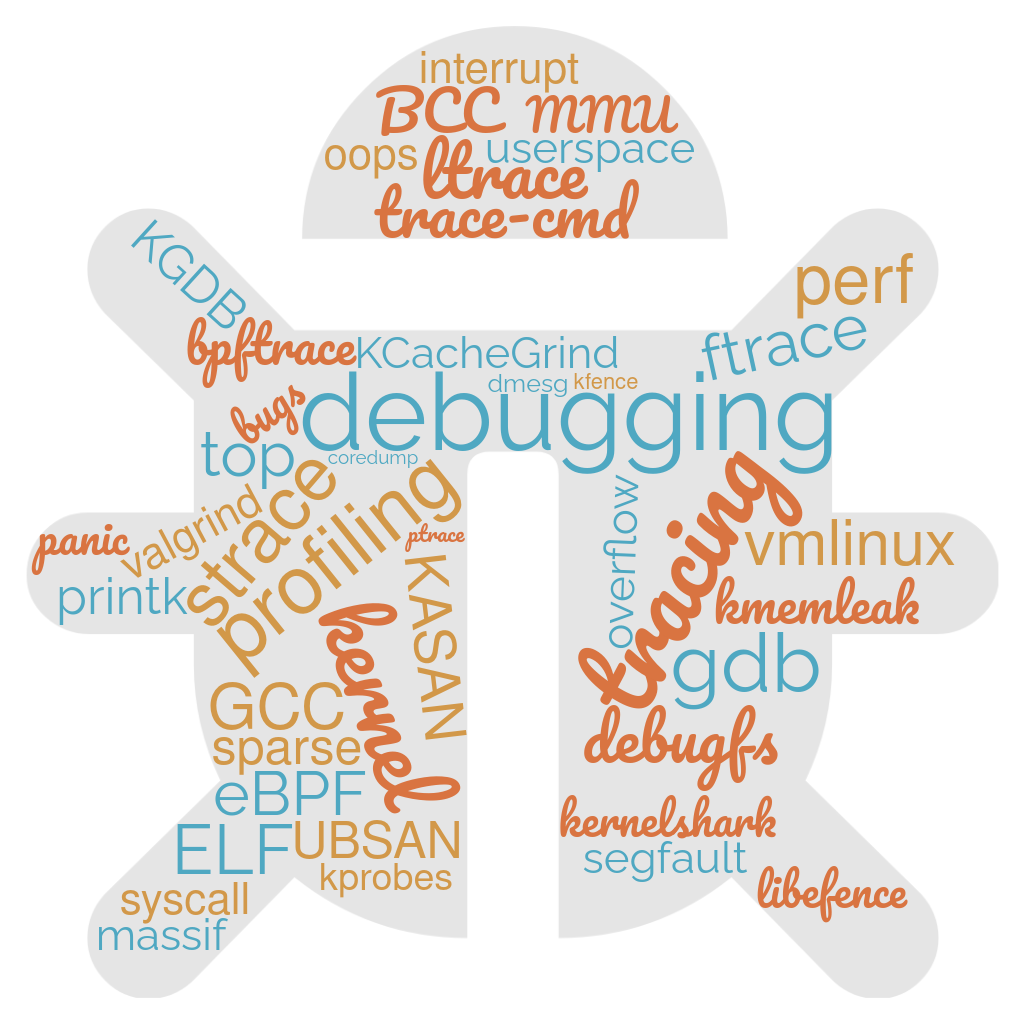
\includegraphics[height=0.6\textheight]{slides/debugging-principles/cloud_word.png}
  \end{columns}
\end{frame}

\begin{frame}
  \frametitle{Debugging}
  \begin{itemize}
    \item Finding and fixing bugs that might exist in your software/system
    \item Use of various tools and methods to achieve that
    \begin{itemize}
      \item Interactive debugging (With GDB for instance)
      \item Postmortem analysis (Using coredump for instance)
      \item Control flow analysis (With tracing tools)
      \item Testing (Targeted tests)
    \end{itemize}
    \item Most commonly done through debuggers in development environnement
    \item Generally intrusive, allowing to pause and resume execution
  \end{itemize}
  \vspace{0.5cm}

  {\small \em "Everyone knows that debugging is twice as hard as writing a program in the first place. So if you're as
    clever as you can be when you write it, how will you ever debug it?" 

  - Brian Kernighan }

\end{frame}

\begin{frame}
  \frametitle{Profiling}
  \begin{itemize}
    \item Analysis at program runtime to assist performance optimizations
    \item Often achieved by sampling counters during execution
    \item Uses specific tools, libraries and operating system features to
          measure performances.
    \begin{itemize}
      \item Using {\em perf}, {\em OProfile} for instance.
    \end{itemize}
    \item First step consist in gathering data from program execution
    \begin{itemize}
      \item Function call count, memory usage, CPU load, cache miss, etc
    \end{itemize}
    \item Then extracting meaningful information from these data and modify the
          program to optimize it
\end{itemize}
\end{frame}

\begin{frame}
  \frametitle{Tracing}
  \begin{itemize}
    \item Following the execution flow of an application to understand the
          bottlenecks and problems.
    \item Achieved by instrumenting code either at compile time or runtime.
    \begin{itemize}
      \item Can be done using specific tracers such as {\em LTTng},
            {\em trace-cmd}, {\em SystemTap} etc
    \end{itemize}
    \item Goes from the user space called functions up to the kernel ones
    \item Allows to identify functions and values that are used while
          application executes
    \item Often works by recording traces during runtime and then visualizing
          data.
    \begin{itemize}
      \item Implies a large amount of recorded data since the complete execution
            trace is recorded
      \item often bigger overhead than profiling.
    \end{itemize}
    \item Can also be used for debugging purpose since data can be extracted
          with tracepoints.
  \end{itemize}
\end{frame}
